\def\alg#1{\texttt{#1}}

\chapter{Implementácia softvéru}\label{chap:implementacia}

V tejto kapitole postupne uvedieme realizáciu návrhu popísaného 
v~kapitole~\ref{chap:popis}. Popíšeme ako sme implementovali jednotlivé 
algoritmy a ukážeme si štruktúru a ovládanie aplikácie. 

% \todo{
% Programovo realizujeme podrobný návrh databázovej aplikácie. 
% Vypracuje sa podrobná dokumentácia k vytvorenému produktu. 
% Vytvorí sa používateľská príručka, kde sa podrobne dokumentuje používateľské rozhranie, spresní sa popis funkcií a spôsob ich aktivácie.
% }

\section{Algoritmy}

Aj keď sme porovnávali iba 10 algoritmov, dokopy bolo implementovaných 
algoritmov viac. V následujúcich častiach postupne uvedieme jednotlivé 
algoritmy a ich označenia pre aplikáciu. Algoritmy boli implementované podľa 
popisu v~kapitole~\ref{chap:algoritmy}.

Pred tým, než rozpíšeme implementáciu algoritmov uvedieme štruktúru a 
implementáciu grafu. Graf je implementovaný ako objekt, ktorý obsahuje 
zoznam hrán. Pokiaľ je to potrebné (čo zväčša je), vie sa iniciovať a zavolať 
vypočítanie susedov do vzdialenosti 2 pre každý vrchol (aby sa nemuselo počítať 
pri každom použití ale iba raz, na začiatku). Taktiež objekt reprezentácie 
grafu vie skontrolovať, či je nejaká množina dominujúcou. To je spravené 
pomocou delegácie na algoritmus kontroly dominujúcej množiny.

Nasleduje popis jednotlivých skupín algoritmov s ich označeniami.

\subsection{Algoritmy skúšajúce všetky možnosti}

Prvým a základným algoritmom je algoritmus, ktorý skúša všetky možnosti. Jeho 
označenie v softvéri je \alg{naive}. Je implementovaný rekurzívnym 
prehľadávaním. Obdobou sú algoritmy označené \alg{mynaive} a \alg{mynaive2}, 
ktoré obsahuje základné heuristiky. Prvou je, že algoritmus najprv zoradí pole 
vrcholov podľa stupňa a až potom začne vyberať do výsledku. Druhou je, že ak 
je medzivýsledok menšej mohutnosti, tak neskúša vyberať množiny s väčšou 
mohutnosťou.

\subsection{Algoritmy prevedenia problému}

Ďalšími algoritmami, ktoré sme implementovali, boli algoritmy, ktoré prevádzali 
hľadanie minimálnej dominujúcej množiny na problém množinového pokrytia. Keďže 
algoritmus bol reprezentovaný návrhovým vzorom \emph{strategy}, tak 
sa implementácia zjednodušila a sprehľadnila. Časť algoritmu sa venovala 
spracovaniu vstupu a časť výpočtu a implementovaniu náročnejších algoritmov. 

Aj keď \citet{fomin05} uvádzajú algoritmus jeden, my sme implementovali dve rôzne 
verzie: \alg{fnaive} a \alg{fproper}. Verzia \alg{fnaive} neobsahuje finálne 
prevedenie na hľadanie minimálneho hranového pokrytia v grafe. Verzia 
\alg{fproper} toto prevedenie obsahuje a implementuje ho cez hľadanie 
maximálneho párenia v grafe. Keďže v čase použitia algoritmu je graf 
bipartitný, tak sa to dá spraviť.

\subsection{Distribuované algoritmy}

Podobne ako predošlé algoritmy, aj tieto algoritmy mali viac verzií. Konkrétne 
jednovláknovú a viacvláknovú. Distribuovanosť bola implementovaná cez veľa 
na sebe nezávislých vlákien. Nedistribuované verzie sme označili príponou 
\alg{-OT} (one thread).

Algoritmy sme implementovali tak ako v prehľade -- dva. Prvý bez riešenia 
problémových grafov (obrázky \ref{img:zle1} a \ref{img:zle2}), ale prehľadnejší 
a zrozumiteľnejší. Druhý s riešením týchto problémov. Prvý je označený ako 
\alg{ch7alg34} (resp.~\alg{ch7alg34OT} pre jednovláknovú verziu) a druhý je 
označený ako \alg{ch7alg35} (podobne \alg{ch7alg35OT} pre jednovláknovú verziu).

\subsection{Pažravé algoritmy}

Keďže jedným z hlavných cieľov práce bolo spraviť dobrú heuristiku na pažravý 
algoritmus, tak boli tieto algoritmy implementované vo viacerých verziách. Okrem 
rôznych heuristík ide aj o spôsob vyberania vrcholov. Počas behu algoritmu sú 
niektoré vrcholy vybraté do medzivýsledku, niektoré pokryté a niektoré 
nevybraté a nepokryté. Tie vrcholy, ktoré sú nevybraté a nepokryté sú 
označované aj ako \emph{biele}, tie ktoré nie sú vybraté, ale sú pokryté sú 
označované ako \emph{šedé} a tie, ktoré sú vybraté sú označované ako 
\emph{čierne}. Na obrázku \ref{img:imp:colors} je znázornené ofarbenie grafu 
po prvom kroku pažravého algoritmu.

\begin{figure}
	\centering
	\greybox{%
		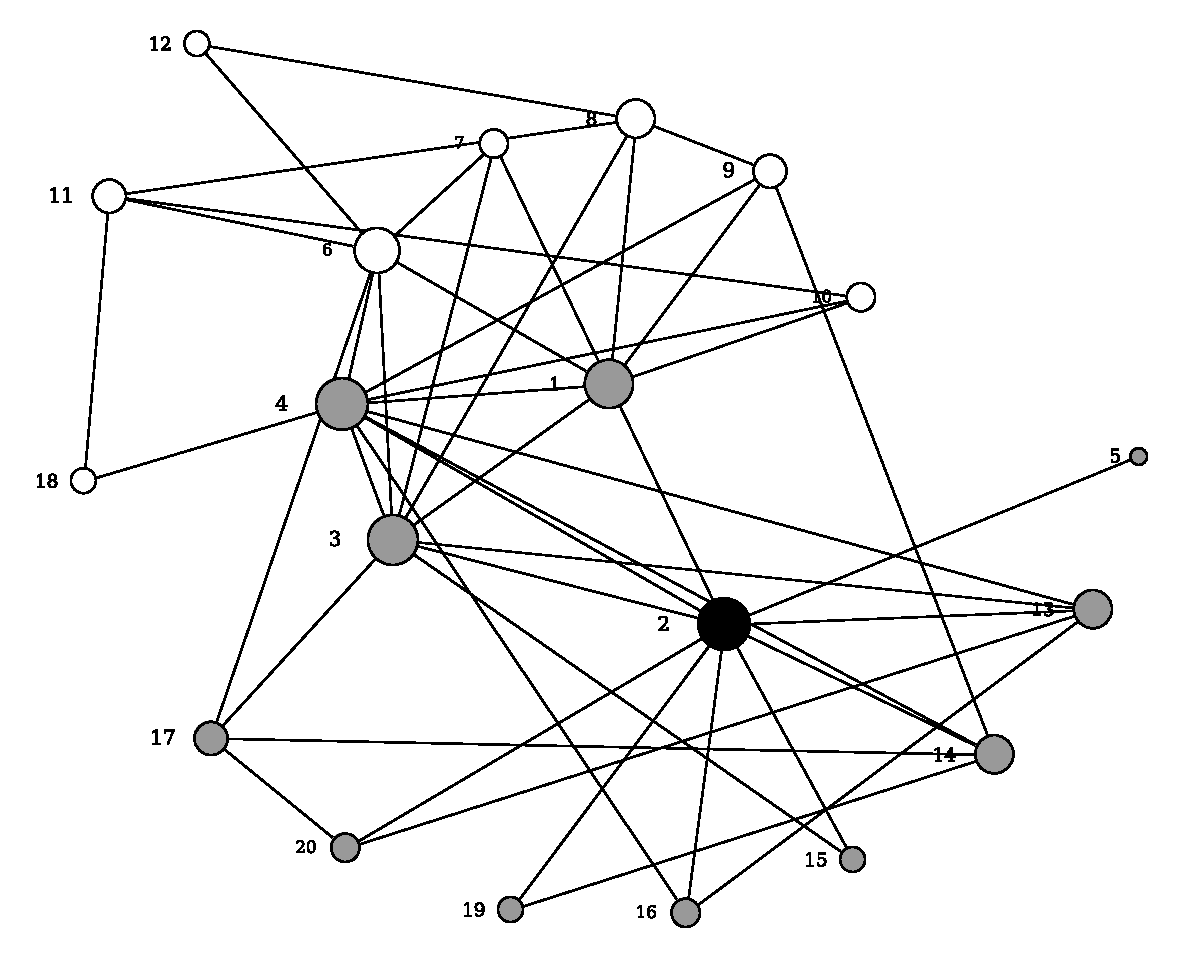
\includegraphics[scale=0.6]{obrazky/colors}%
	}
	\caption{\emph{Príklad prvého kroku pažravého algoritmu.} 
	Vrcholy v grafe majú veľkosť úmernú stupňu (čím väčší stupeň, tým väčší 
	priemer vrchola). V prvom kroku si algoritmus mohol vybrať vrchol 2, čím ho 
	označil ako čierny a jeho susedov (tým dominuje) označil šedou farbou. 
	Bielou sú označené vrcholy, ktoré ešte nie sú dominované čiernymi.}
	\label{img:imp:colors}
\end{figure}


Podľa algoritmu, ktorý je uvedený v časti \ref{sec:greedy} sme implementovali 
algoritmus, ktorý sme označili \alg{greedy}. Podobne sme implementovali aj 
verziu \alg{ch7alg33}. Avšak tá nevyberá vrcholy, ktoré pokrývajú čo najviac 
iných spomedzi šedých a bielych, ale iba z bielych vrcholov. Veľmi podobne je 
implementovaná aj verzia \alg{greedyq}. Jediný rozdiel je, že vrcholy na 
začiatku behu usporiada podľa stupňa od najväčšieho po najmenší.

\subsubsection{Heuristiky na rozhodovanie}

Po troch podobných verziách sme implementovali rôzne heuristiky. Prvou bolo 
odstraňovanie výhonkov. Toto odstraňovanie prebieha na začiatku 
algoritmu, postupne v iteráciách, až kým nie je čo odstrániť. Motiváciou za 
týmto algoritmom je efektívne odstraňovanie ciest. Verzia algoritmu s touto 
heuristikou je označovaná ako \alg{greedysr}. 

V ďalšej verzii sme použili opäť základný pažravý algoritmus, ale ako 
rozhodovací faktor pre výber vrchola sme vybrali počet vrcholov, ktoré po 
vybratí už nebudú mať bieleho suseda (toto nie je to isté ako rád kveta) 
a až potom počet vrcholov, ktorým vrchol dominuje. Motiváciou bolo 
presvedčenie, že často je lepšie vybrať vrchol, ktorý po svojom vybratí čo 
najviac zmenší počet potenciálne vybratých vrcholov v ďalších iteráciách, 
namiesto vyberania vrcholov s najväčším pokrytím.
Heuristika by mala byť nejakým 
kompromisom medzi vyberaním vrcholov "zospodu" a "zvrchu". Táto verzia 
algoritmu je označená ako \alg{greedysw}.

\subsubsection{Zložitejšia heuristika}

Treťou verziou je \alg{floweru}, ktorá je podobná ako \alg{greedysr}, s tým 
rozdielom, že na začiatku spraví iba jeden beh odstraňovania výhonkov. Toto je 
základom pre posledný, zložitejší algoritmus, ktorý je označený \alg{flower}. 

Verzia \alg{flower} na začiatku behu zoradí vrcholy podľa stupňa. Následne sa 
snaží označiť výhonky a kvety. Vyčistí výhonky a upraví graf tak, aby sa mohli 
vybrať kvety. Kvety sa vyberajú postupne. Najviac záleží na ráde kvetu. Ak majú 
nejaké kvety rovnaký rád, tak sa rozhoduje podľa toho, koľko vrcholov po 
vybratí už nebude mať bieleho suseda (podobne ako pri verzii \alg{greedysw}). 
Ak je aj táto hodnota rovnaká, tak zaváži počet bielych susedov (najväčšie 
pokrytie). Ak nepomôže ani toto pravidlo, tak sa vyberie náhodný vrchol.

Po označení výhonkov a kvetov sa začnú označovať zvyšné vrcholy podľa 
jednoduchého pažravého algoritmu. Avšak ako rozhodujúci faktor pri vyberaní 
slúži najprv počet bielych susedov (pokrytie) a potom počet vrcholov, ktoré 
po vybratí už nebudú mať bieleho suseda.

\subsection{Dátové štruktúry a externé knižnice}

Aj keď na porovnanie rôznych algoritmov sú základné dátové štruktúry 
poskytované ako súčasť knižníc jazyka \Java, rozhodli sme sa použiť na 
implementáciu základných dátových štruktúr knižnicu HPPC od poskytovateľa 
Carrot Search Labs vo verzii 0.6.0. Je dostupná na webovej adrese 
\url{http://labs.carrotsearch.com/hppc.html} a licencovaná Apache License 2.0. 
hlavnou výhodou knižnice oproti štandardnej knižnici je menšia spotreba pamäte 
a priamejší prístup k vnútornej reprezentácií (aspoň v danej verzii). To 
spôsobilo celkové zrýchlenie algoritmov a posunulo hranice testovateľných 
grafov.

Aj keď medzi analyzovanými existujúcimi riešeniami je veľa grafových knižníc, 
pripadalo nám jednoduchšie a efektívnejšie implementovať vlastnú reprezentáciu 
grafov pomocou základných prvkov jazyka \Java\ a knižnice HPPC.


